%%%%%%%%%%%%%%%%%%%%%%%%%%%%%%%%%%%%%%%%%%%%%%%%%%%%%%%%%%%%%%%%%%%%%%%%%%%%%%%%
%2345678901234567890123456789012345678901234567890123456789012345678901234567890
%        1         2         3         4         5         6         7         8

\documentclass[letterpaper, 10 pt, conference]{ieeeconf}  % Comment this line out if you need a4paper

%\documentclass[a4paper, 10pt, conference]{ieeeconf}      % Use this line for a4 paper

\IEEEoverridecommandlockouts                              % This command is only needed if 
                                                          % you want to use the \thanks command

\overrideIEEEmargins                                      % Needed to meet printer requirements.

%In case you encounter the following error:
%Error 1010 The PDF file may be corrupt (unable to open PDF file) OR
%Error 1000 An error occurred while parsing a contents stream. Unable to analyze the PDF file.
%This is a known problem with pdfLaTeX conversion filter. The file cannot be opened with acrobat reader
%Please use one of the alternatives below to circumvent this error by uncommenting one or the other
%\pdfobjcompresslevel=0
%\pdfminorversion=4

% See the \addtolength command later in the file to balance the column lengths
% on the last page of the document

% The following packages can be found on http:\\www.ctan.org
\usepackage{graphics} % for pdf, bitmapped graphics files
\usepackage{epsfig} % for postscript graphics files
\usepackage{mathptmx} % assumes new font selection scheme installed
\usepackage{times} % assumes new font selection scheme installed
\usepackage{amsmath} % assumes amsmath package installed
\usepackage{amssymb}  % assumes amsmath package installed

\usepackage{hyperref}
\usepackage{url}
\usepackage{tabularx}
\usepackage{multirow}
\usepackage{booktabs}
\usepackage{pifont}
\usepackage{algorithm}
\usepackage{algorithmic}
\usepackage{makecell}
\usepackage{xcolor}
\usepackage{caption}
% \usepackage[font=footnotesize]{caption}
\usepackage{siunitx}
\usepackage{xspace}

\renewcommand{\baselinestretch}{0.98}

\newcommand{\karen}[1]{\textbf{\color{red}[Karen: #1]}}
\newcommand{\guanya}[1]{\textbf{\color{cyan}[Guanya: #1]}}
\newcommand{\zhen}[1]{\textbf{\color{brown}[Zhen: #1]}}
\newcommand{\lujie}[1]{\textbf{\color{purple}[Lujie: #1]}}
\newcommand{\ak}[1]{\textbf{\color{blue}[AK: #1]}}
\newcommand{\rocky}[1]{\textbf{\color{blue}[Rocky: #1]}}
\newcommand{\carlo}[1]{\textbf{\color{orange}[Carlo: #1]}}
\newcommand{\OmniRetarget}{\textsc{OmniRetarget}\xspace}

\title{\LARGE \bf
OmniRetarget: Interaction-Preserving Data Generation for Humanoid Whole-Body Loco-Manipulation and Scene Interaction
}

% Authors: Lujie*, Xiaoyu*, Zhen*, Russ?, Angjoo+, Pieter+, Carlo+, Karen+, Rocky+, Guanya+

\author{Lujie Yang*$^{1, 2}$, Xiaoyu Huang*$^{1, 3}$, Zhen Wu*$^{1}$, \\ Angjoo Kanazawa$^{\dagger 1, 3}$, Pieter Abbeel$^{\dagger 1, 3}$, Carmelo Sferrazza$^{\dagger 1}$, C. Karen Liu$^{\dagger 1, 4}$, Rocky Duan$^{\dagger 1}$, Guanya Shi$^{\dagger 1, 5}$ \\
$^{1}$Amazon FAR (Frontier AI \& Robotics), $^{2}$MIT, $^{3}$UC Berkeley, $^{4}$Stanford University, $^{5}$CMU %
\thanks{* Equal contribution, work done while interning at Amazon FAR. $\dagger$ Amazon FAR team co-lead.}% <-this % stops a space
% \thanks{}%
% \thanks{$^{2}$Bernard D. Researcheris with the Department of Electrical Engineering, Wright State University,
%         Dayton, OH 45435, USA
%         {\tt\small b.d.researcher@ieee.org}}%
% }
}

\newcommand{\yes}{\textcolor{green}{\ding{51}}}
\newcommand{\no}{\textcolor{red}{\ding{55}}}

\DeclareMathOperator*{\argmin}{arg\,min}

% hook into \@maketitle to add the wanted figure
\AddToHook{cmd/@maketitle/after}{\ADDINITIALFIGURE}
% the code for the figure
\newcommand{\ADDINITIALFIGURE}{%
  % we want to emulate a fixed float
  \begin{minipage}{\textwidth}
    % pretend we're inside figure
    \expandafter\def\csname @captype\endcsname{figure}%
    \centering
    \includegraphics[width=\textwidth]{figures/teaser_v3.3.pdf}%
    % the text is processed a few times, so we reset the counter each time
    \setcounter{figure}{0}
    \captionof{figure}{
    \OmniRetarget enables reinforcement learning policies to learn complex, long-horizon loco-manipulation skills in challenging environments that transfer zero-shot from simulation to a Unitree G1 humanoid. Thanks to the high-quality interaction-preserving motion retargeting, these policies are trained and deployed in a \emph{minimal and unified} way: it involves only 5 rewards, 4 robot domain randomization terms, and a purely proprioceptive observation space, shared by all tasks. Demonstrated behaviors include \textbf{(a)} 30-second parkour course involving chair moving, stepping \& vault, and jump \& roll, \textbf{(b)} object transportation, \textbf{(c)} crawling on a slope, and \textbf{(d)} fast platform climbing and sitting. 
    % \guanya{@Zhen, could you add abcd on the figure? Also add a rough vel on d to emphasize the speed} \zhen{updated}
    \label{fig:flagship_demo}}
  \end{minipage}}
  
\begin{document}

\maketitle
\thispagestyle{empty}
\pagestyle{empty}


\begin{abstract}

% 1. Excel complex
% 2. rely on human
% 3. Save how much effort


% v2

Excel is one of the most widely used productivity tools across domains, offering rich functionality but also overwhelming users with its complexity. This creates a persistent demand for tutorials to support effective usage. However, existing tutorials are manually authored by experts, require frequent updates after each software release, and incur substantial labor costs. Prior work has not achieved fully automated tutorial generation, since existing methods still depend on handcrafted operation sequences or example materials.
In this paper, we present the first framework for automatically generating Excel tutorials directly from natural language task descriptions. Our framework first instantiates the task. Then a central component of this framework, Execution Agent, plans and executes the solution in Excel, and collects the intermediate artifacts required for tutorial construction. These artifacts are then transformed into both structured Excel documents and video demonstrations. To build a comprehensive tutorial corpus, we collected 1,559 task descriptions from real-world scenarios. In addition, we designed a systematic evaluation framework that integrates assessments from both large language models (LLMs) and human reviewers. Experimental results show that our framework improves task execution success rates by 8.5\% over state-of-the-art baselines. Moreover, the generated tutorials demonstrate superior readability and instructional effectiveness, often approaching or surpassing expert-authored materials. Importantly, the automated pipeline eliminates manual labor and reduces time costs to 1/20 of expert authoring, making scalable and high-quality tutorial generation practical for the first time.


% v1
% Excel is extensively adopted across diverse domains due to its rich functionality and broad user base. However, its complex and heterogeneous features often overwhelm users, creating a strong demand for tutorials as a source of support and guidance. Existing tutorials are predominantly authored by experts and require frequent manual updates following each software release, resulting in substantial labor costs. Prior research has not achieved fully automated tutorial generation, as existing approaches still rely on manually curated operation sequences and example materials. Consequently, the automatic generation of high-quality tutorials remains an open and challenging problem. In this paper, we present the first framework capable of automatically generating Excel tutorials directly from task descriptions. Our framework first instantiates the task, then plans and executes the corresponding solution while collecting the materials required for tutorial construction. Finally, these materials are transformed into both Excel documents and video tutorials. To build a comprehensive tutorial corpus, we collected 1,559 task descriptions from real-world scenarios. In addition, we designed a systematic evaluation framework that integrates assessments from both large language models (LLMs) and human reviewers. Experimental results demonstrate that, compared to state-of-the-art baselines, Excel Guide Agent improves task execution success rates by 8.5\%. In terms of tutorial quality, the generated tutorials exhibit superior readability and instructional effectiveness, approaching or even surpassing the level of expert-authored materials. Importantly, the automated process eliminates manual labor and reduces time costs to 1/20 of expert authoring.



% v0
% Excel is widely used across diverse scenarios due to its rich functionality \cz{but complex?}  and a large user base. As users face increasingly complex and diverse Excel features, Excel tutorials have become more and more important. Existing Excel tutorials \cz{rely on human?} (1) incur substantial labor costs for authoring and maintenance and (2) exhibit limited task coverage. Therefore, there is an urgent need for automated solutions to generate more comprehensive Excel tutorials with high quality and low cost. In this paper, we first formalize the task to tutorial problem, supported by a evaluation protocol and a dataset of 1,559 Excel tasks. We then introduce \textbf{Excel Guide Agent}, the first framework capable of automatically generating Excel tutorials (including help
% documents and videos) solely from task descriptions. 

% This framework enables end-to-end generation from task to tutorial via three stages: (1) instantiating tasks by matching Excel templates based on task descriptions, (2) performing solution planning and execution via a task executor, and (3) generating tutorial components and assembling them into multimodal, multi-format tutorials.
% We conducted extensive experiments on real-world Excel tasks from diverse sources, under three base model configurations (GPT-4.1, GPT-o3, GPT-5). \cz{too detailed...} Experimental results demonstrate that, compared with state-of-the-art models, Excel Guide Agent improves task execution success rate by 8.5\%. Human and LLM evaluations confirm that our tutorials demonstrate excellent readability and instructional effectiveness, and can even surpass those written by domain experts. Furthermore, we have constructed a more comprehensive Excel tutorial library using Excel Guide Agent at low cost. \cz{Save how much effort?}
\end{abstract}



% \section{Introduction}
% \fix{finish}\cz{Story: Excel is popular but complex, rely on tutorial. Current tutorials are hand-crafted, not scalable. Motivate us to auto-generate ... With LLM and Agent, this may become feasible, but still challenging because ... To solve these challenges, we xxx}

% Excel offers a wide range of functionalities and is a extensively used across various domains, including finance, analytics, and science research~\cite{chan1996use, hacker2017financial, powell2019business}.
% While numerous online tutorials exist, they are typically authored by professionals or domain experts, resulting in high labor costs and limited coverage of frequently asked questions (FAQs). Moreover, as software continues to evolve, these tutorials require ongoing manual maintenance. Without such maintenance, operational details may become outdated or inconsistent, and accompanying screenshots may no longer reflect the current interface. This significantly increases the cost of tutorial development and upkeep. Given the critical role of tutorials and the limitations of manual creation in terms of scalability and coverage, there is a pressing need for a fully automated framework capable of generating tutorials directly from tasks.


% To reduce the manual effort required for producing high-quality tutorials, prior work has proposed techniques for semi-automated tutorial generation. Several approaches aim to automatically create tutorials based on expert demonstrations~\cite{chi2012mixt, grabler2009generating} or existing user manuals~\cite{liu2024having, zhong2021helpviz}. These methods primarily focus on augmenting pre-existing instructional content—for example, transforming user manuals into instructional videos—to enhance understanding and improve visualization. However, all of these approaches rely on solutions provided by experts, making it impossible to generate tutorials in a fully end-to-end manner.


% Recent advances in Large Language Models (LLMs) and agent systems have made the vision of automated tutorial generation increasingly feasible. For example, sheet agents can automate a wide range of spreadsheet operations. However, their reliance on code execution renders the process opaque to end users, failing to provide a UI-based learning pathway. Similarly, Computer-Using Agents (CUAs) can automatically plan application-level tasks and simulate human interactions to complete them. Yet, applying CUAs to Excel remains challenging due to the application’s densely structured interface and the fine-grained nature of its operations (e.g., cells, borders, and other components). Generating tutorials from task descriptions further compounds this difficulty, as it requires not only task planning and execution but also material collection and tutorial construction. To date, no existing LLM or agent framework can support this end-to-end process.


% In this work, we aim to generate comprehensive procedural steps for Excel with documents and videos automatically. Documents present a sequence of steps, each accompanied by textual descriptions and, in some cases, one or more images~\cite{zhong2021helpviz}. Demonstration videos are recorded by professionals and feature audio narration~\cite{torrey2007pages,tuncer2020pause}, which further benefit viewers who prefer auditory guidance while observing actions~\cite{tuncer2020pause}. Different formats offer distinct learning benefits: documents are efficient for quickly skimming a procedure, and videos are effective for demonstrating the exact execution of a task, especially when presented in a step-by-step manner~\cite{chi2012mixt,truong2021automatic,zhu2021gif}. 

% We first formalize the task of Excel tutorial generation: create step-by-step tutorials with documents and videos, given an Excel task. 
% To comprehensively evaluate the effectiveness of our methods, we build a dataset comprising 1,559 real-world Excel tasks covering 28 categories of operation types and 17 categories of target objects. Compared with existing Excel manipulation datasets, our dataset includes Excel-level tasks that are absent in prior work and offers broader coverage of spreadsheet-level tasks.
% On this foundation, we present the first automated Excel tutorial framework that executes Excel tasks and produces both instruction documents and videos. Our framework consists of three core modules: (1) task instantiation, (2) automatic trajectory collection, and (3) tutorial generation. Specifically, in the task instantiation module, queries from collected datasets are rewritten to be clear tasks in Excel and each task will be matched with a suitable Excel file for tutorial generation as no execution files are available in the original datasets.
% Then, the sequence of actions is generated in the automatic trajectory collection module, simulating the behavior of human experts. The Execution Agent determines each subsequent step based on the current screenshot and the history of prior actions. Finally, instructional documents and videos are created based on the action sequence in the Tutorial Generation module.
% For each step, the system generates a concise, user-friendly title and description, linked with the corresponding screenshots and action video. 


% To comprehensively evaluate the quality of generated instructional documents and videos, We adopts both human experts rates and MLLMs as judges with an evaluation protocol that scores the candidate tutorials on complementary criteria (see \autoref{sec:eval_metrics}). The experiment results show that our method can produce high-quality instruction documents and videos that effectively guide users in completing their tasks.
% The main contributions of this work are as follows:
% \begin{itemize}
%     \item We propose a novel pipeline for automatically generating Excel tutorials from task descriptions. To the best of our knowledge, this is the first work that enables tutorial creation solely based on task inputs.
%     \item We propose an Execution Agent (ExeAgent), which produces and executes the operation sequences required to complete Excel tasks. The success rate of task executor hits 39.58\% success rate, surpassing existing state-of-the-art approaches.
%     \item We propose a diverse and representative dataset consist of Excel tasks from multiple sources and generate tutorials across various types. The resulting tutorials covers a wide range of operation categories and target users, meeting learning needs in different scenarios while maintaining accuracy and practicality. Notably, our approach eliminates manual labor, requiring only one-twentieth of the time cost compared to expert-authored tutorials. %\cz{Save how many effort?}
%     \item We design a systematic set of evaluation metrics and conducted human evaluations. The results indicate that our method generates high-quality instructional content and effectively guides users in completing Excel-related tasks.
% \end{itemize}

% \fix{finish}\cz{1. Auto generate pipeline, 2. design xx agent, better successful rate 3. with real data, auto generate xxx video and tutorial 4. Human evaluation suggests that xxx, and save xxx effort.}
\section{Introduction}

Excel provides a comprehensive set of functionalities and is extensively adopted across domains such as finance, analytics, and scientific research~\cite{chan1996use,hacker2017financial,powell2019business}. 
Its versatility makes it a critical tool for data management, statistical analysis, and visualization. 
At the same time, this richness of features creates significant learning barriers, as many users struggle to identify the appropriate operations or to integrate multiple functions effectively~\cite{carroll1990nurnberg,ko2007information}. 
To mitigate these challenges, tutorials have long served as an essential support mechanism, guiding users through common tasks and enabling more effective utilization of Excel’s capabilities.
However, existing tutorials are predominantly authored by domain experts, which entails substantial labor costs and restricts coverage across the diverse range of tasks users encounter~\cite{grossman2010toolclips}.
Moreover, as software evolves, these tutorials must be continuously updated: outdated screenshots, obsolete descriptions, and inconsistent workflows reduce their instructional value~\cite{liu2024having}. 
This dependence on manual authoring highlights the need for a scalable, automated approach to tutorial generation.

Prior research has explored semi-automated methods for tutorial creation. 
Some approaches generate tutorials based on expert demonstrations~\cite{chi2012mixt,grabler2009generating}, while others transform existing manuals into instructional videos or annotated guides~\cite{liu2024having,zhong2021helpviz}. 
Although these methods improve efficiency, they fundamentally rely on curated expert solutions, preventing a fully end-to-end pipeline. 
Recent advances in large language models (LLMs) and agent systems make automated tutorial generation increasingly feasible~\cite{zhang2024ufo,liu2025infigui}. 
Spreadsheet agents can already automate a variety of operations~\cite{li2023sheetcopilot}, but their code-driven execution remains opaque to end users, offering limited pedagogical benefit. 
Similarly, Computer-Using Agents (CUAs) ~\cite{openai2025computer,zhang2025ufo2} demonstrate the ability to plan application-level tasks through simulated human interactions. 
However, applying such systems to Excel is uniquely challenging due to its densely structured interface and fine-grained operations (e.g., cell editing, formulas, and borders). 
Generating tutorials from task descriptions adds an additional layer of difficulty: the system must not only plan and execute tasks but also collect execution traces, screenshots, and contextual information suitable for tutorial construction. 
To date, no existing work addresses this end-to-end requirement.

In this paper, we present the first framework for automatically generating Excel tutorials directly from natural language task descriptions. Our framework first instantiates the task. Then the Execution Agent plans and executes the solution in Excel, and collects the intermediate artifacts required for tutorial construction. These artifacts are subsequently transformed into step-by-step instructional documents and narrated video demonstrations. 
Different tutorial formats offer complementary learning benefits: documents allow for efficient skimming of procedures, while videos provide clear demonstrations of fine-grained execution steps and are particularly useful for users who prefer visual or auditory guidance~\cite{torrey2007pages}. 

To support development and evaluation, we curate a dataset of 1,559 real-world Excel tasks spanning 28 operations and 17 target object categories. 
This dataset covers Excel-level tasks absent from prior work and enables comprehensive tutorial generation at scale. 
We further design a systematic evaluation protocol that combines human expert judgments with LLM-based assessments. 
Experimental results show that our framework improves execution success rates by 8.5\% over state-of-the-art baselines. 
Moreover, the generated tutorials demonstrate superior readability and instructional effectiveness, often approaching or surpassing expert-authored materials, while reducing authoring costs to one-twentieth of manual effort. 
Our main contributions are as follows:
\begin{itemize}
    \item We propose the first end-to-end framework for generating Excel tutorials directly from natural language task descriptions, producing both instructional documents and video demonstrations. 
    \item We introduce an Execution Agent that plans and executes Excel tasks while collecting intermediate artifacts for tutorial generation, achieving a task execution success rate of 39.58\% and surpassing state-of-the-art baselines. 
    \item A diverse dataset of 1,559 real-world Excel tasks is curated, covering a wide range of operations  and target object categories to enable scalable and representative tutorial generation. 
    \item A systematic evaluation protocol is designed with both human and LLM-based judges, demonstrating that the generated tutorials are effective, readable, and substantially reduce manual labor costs. 
\end{itemize}


\section{Related Works}
\subsection{Motion Retargeting}\label{sec:motion_retargeting}
In computer graphics, transferring motions across characters has been extensively explored. Researchers have employed optimization-based methods to retarget human motions to avatars by preserving distances and orientations between keypoints \cite{cheynel2023sparse}, minimizing deformation energy \cite{Ho2010Spatial, kim2016retargeting}, or scaling the motions to satisfy hard constraints \cite{gleicher1998retargetting}. Others leverage data-driven methods that map diverse skeletons to a canonical representation \cite{aberman2020skeleton}, solve inverse kinematics with neural networks \cite{villegas2018neural}, or use reinforcement learning to preserve an interaction graph \cite{zhang2023simulation}.

% Retargeting motions for physical humanoid robots introduces challenges beyond character animation, most notably the need to enforce physical constraints. A direct adaptation of a graphics method PHC \cite{Luo2023PerpetualHC}, widely used in RL training \cite{he2025asap, chen2025gmt, he2024omnih2o}, which uses a common approach of, keypoint matching, minimizes key body distances to human demonstrators but could violate physical constraints. solves an unconstrained optimization, yielding motions with interpenetration, foot skating, and no awareness of objects or environments. 
Retargeting motions to humanoid robots introduces challenges beyond character animation, particularly the need to enforce physical constraints. For example, PHC \cite{Luo2023PerpetualHC}, a graphics method adopted in robotics~\cite{he2025asap, he2024omnih2o}, uses keypoint matching with unconstrained optimization, often leading to penetration, foot skating, and lack of object or scene awareness.
Similarly, GMR~\cite{ze2025twist} extends keypoint matching to orientations but suffer the same issues. 
VideoMimic~\cite{videomimic} improves realism with soft contact and collision penalties but offers no guarantees and requires careful tuning.

The closest method to ours is Interaction Mesh based Motion Adaptation (IMMA) \cite{Nakaoka2012Interaction}, which also leverages an interaction mesh \cite{Ho2010Spatial} to preserve the spatial relationship between body parts. However, it is not open-sourced and ignores kinematic limits and interactions with the environment or manipulated objects. 
In contrast, \OmniRetarget unifies all hard constraints, including foot sticking, non-penetration, and joint and velocity limits, while explicitly preserving environment and object interactions.

\subsection{Learning-Based Humanoid Whole-Body Control}
% margolis2023walk xie2018feedback
% \guanya{\begin{itemize}
%     \item Humanoid WBC learning is promising
%     \item Motion tracking methods have advanced, levearing data... (Fousing on flat terrian)
%     \item Few work extent do interaction setting
%     \item In summary, all these methods lack XXX
% \end{itemize}}

Recent learning-based whole-body control has enabled humanoids to traverse dynamic scenes and manipulate objects~\cite{dao2024sim, long2024learning, he2025attention, he2025learning, kuang2025skillblender, zhang2025unleashing, xue2025unified, zhang2406wococo, zhang2025falcon}. These methods typically train with hand-crafted rewards or task interfaces (e.g., velocity tracking, contact schedules, end-effector targets) but depend on extensive reward engineering and mostly fail to yield natural, human-level motions.
% These interfaces enable a wide range of behaviors, including getting up from the ground, stepping stones, predefined locomotion gaits with upper body movements, scene traversal, and object manipulation. Yet, these methods typically require extensive reward engineering and still struggle to produce natural, expressive motions that achieve human-level agility and behavior. 

Motion imitation offers a promising alternative. In graphics, DeepMimic~\cite{peng2018deepmimic} shows that using human references yields natural, human-like behaviors with agile, dynamic motions. 
However, applying this approach to humanoid robots remains difficult due to the lack of reliable open-source kinematic retargeting pipelines.
With suboptimal reference motions, practitioners are forced to either manually clean the data~\cite{zhang2025hub} or re-introduce extensive reward engineering, such as ad-hoc regularizers for contact, slipping, and air time, to compensate for artifacts~\cite{ze2025twist, he2025asap, li2025reinforcement}. In contrast, trackers with minimal reward formulation like BeyondMimic~\cite{liao2025beyondmimic} achieve state-of-the-art results on hardware with high-fidelity references~\cite{unitree_lafan1_retargeting_dataset}, but those are scarce and robot-only, without interactions.

Beyond single-character motion, human–scene interaction data has proven effective for terrain traversal and loco-manipulation in character animation~\cite{xu2025parc, wu2024human}, but translating this to robotics remains challenging. 
VideoMimic~\cite{videomimic} applies this idea to human–terrain traversal by reconstructing motions and terrains from video, but suffers from artifacts and is limited to static–scene interactions. To bridge this gap, \OmniRetarget enables natural, agile robot-object-scene interactions with high-quality reference from retargeting without manual post-processing or reward engineering.
% Beyond single-character motion, human–scene interaction data has also proven effective for terrain traversal and loco-manipulation in character animation~\cite{xu2025parc, wu2024human}.  
% However, translating this success to robotics has proven challenging.
% One of the prior works, VideoMimic~\cite{videomimic}, applies this approach to human-terrain traversal by reconstructing motions and terrains from video, but suffers from limited quality and diversity due to reconstruction and retargeting artifacts. Furthermore, their approach only deal with static environment and does not address human-object interactions. 
% Bridging this gap, \OmniRetarget enables natural and agile robot-scene interactions by tracking high-quality reference motions without manual post-processing or reward engineering.

\subsection{Data Generation for Humanoid Loco-Manipulation}
% The demand for large-scale data to train versatile whole-body loco-manipulation policies has motivated a variety of data generation strategies. 
The demand for whole-body interaction data has motivated many prior works on data generation.
One approach is direct human teleoperation \cite{seo2023deep, fu2024humanplus, he2024omnih2o, ze2025twist, ben2025homie}. While it provides online feedback, teleoperation is difficult to scale: it's labor-intensive, prone to operator fatigue, and limited by the embodiment gap between human and robot kinematics. The lack of rich haptic feedback and difficulty stabilizing extreme motions (e.g., deep squats) further constrain its applicability. To address these scaling challenges, automated data augmentation has been explored, particularly for robotic manipulation. Many works leverage state-of-the-art generative models for visual \cite{zhang2024diffusion, tian2024view, chen2024rovi} and semantic \cite{mandi2022cacti, chen2023genaug, yu2023scaling} augmentations, while others rely on simple open-loop kinematic replay of base trajectories  \cite{mandlekar2023mimicgen, jiang2024dexmimicgen, garrett2024skillmimicgen} or trajectory optimization \cite{yang2025physics} in simulation. 
Despite the advances in manipulation, data augmentation for whole-body loco-manipulation remains largely unexplored. 
The closest prior work~\cite{starke2019neural} interpolates keypoints to augment objects of different shape, but it cannot deal with varied object poses either. 
\OmniRetarget directly addresses this gap.


% \vspace{-0.05cm}
\section{Interaction-Preserving Motion Retargeting}
% \begin{table}[h!]
% \centering
% \small
% \renewcommand{\arraystretch}{1.3}
% \begin{tabularx}{\textwidth}{l *{4}{>{\centering\arraybackslash}X} l}
% \toprule
% Methods & Prevent Foot Skating & Non-penetration & Preserve Interaction w/ Object & Data Augmentation & Optimizer \\
% \midrule
% PHC & \no & \no & \no & \no & Gradient Descent \\
% GMR & \no & \no &\no & \no & Mink ~\cite{Zakka_Mink_Python_inverse_2025}\\
% VideoMimic & Soft penalty & Soft penalty & \no & \no & \makecell[t]{JAX Levenberg-\\Marquardt}\\
% IMMA & \yes & \yes & \no & \no & Lagrange Method\\
% \OmniRetarget (Ours) & \yes & \yes & \yes &\yes & SQP \\
% \bottomrule
% \end{tabularx}
% \caption{Comparison of retargeting methods across constraint enforcement, interaction preservation, data augmentation and optimization strategy.}
% \end{table}
\begin{table*}[t]
\centering
\footnotesize
\renewcommand{\arraystretch}{1.15}
\setlength{\tabcolsep}{4pt}
\begin{tabularx}{\textwidth}{l *{5}{>{\centering\arraybackslash}X} l}
\toprule
\textbf{Methods} & \textbf{Hard Kinematic Constraints} & \textbf{Interaction w/ Object} & \textbf{Interaction w/ Terrain} & \textbf{Data Augmentation} & \textbf{Optimization Method} \\
\midrule
IMMA~\cite{Nakaoka2012Interaction}  & \yes & \no & \no & \no & QP \\
PHC~\cite{Luo2023PerpetualHC} & \no & \no & \no & \no & Gradient Descent \\
GMR~\cite{ze2025twist}  & \no & \no & \no & \no & Mink~\cite{Zakka_Mink_Python_inverse_2025} \\
VideoMimic~\cite{videomimic}  & Soft Penalty & \no & \yes &\no & JAX L-M \\
\midrule
\textbf{\OmniRetarget (Ours)}  & \yes & \yes & \yes &\yes & Sequential SOCP \\
\bottomrule
\end{tabularx}
\caption{Comparison of prior retargeting methods across different aspects.}
\label{tab:retargeting_comparison}
% \vspace*{-0.4cm}
\end{table*}

%Levenberg-\\Marquardt

% IMMA relies on a complex, multi-stage pipeline: first, it optimizes keypoint positions to warp the interaction mesh from the human to the robot with minimal deformation; then, it solves an inverse kinematics problem to recover joint angles that best match the optimized keypoints. In later stages, additional hard constraints on the feet and waist are imposed to prevent foot slipping and ensure dynamic balancing. This sequential and fragmented approach produces dynamically consistent motions but 
 % \karen{This is what a reviewer might say: It sounds like the proposed method and IMMA can achieve the same thing and the only difference is that your method has a better implementation. I think we put too much effort in describing how IMMA works which dilutes the most important sentence: IMMA fails to enforce joint and velocity limits and does not support interactions with the environment and objects. We should say that right after "However". }.

\subsection{Interaction Mesh with Hard Constraints}
We leverage the interaction mesh \cite{Ho2010Spatial} to preserve spatial relationships between body parts, objects, and the environment. The interaction mesh is defined as a volumetric structure whose vertices consist of key robot or human joints together with points sampled from objects and the environment. By shrinking or stretching this mesh, we can warp human motion onto the robot while preserving relative spatial configurations and contact relationships.  

\textbf{Interaction Mesh Construction.}  
We construct the interaction mesh by applying Delaunay tetrahedralization \cite{si2005meshing} to user-defined key joint positions and randomly sampled object and environment points. To more accurately maintain contact relationships, we sample the object and environment surfaces more densely than the body joints. 
% \guanya{I think we need a humanoid example to illustrate it}
% \karen{Reviewer might wonder why we need to do Delaunay triangularization every frame. Even if we are solving frame by frame, the connectivity of the interactive mesh can remain across frames.}

\textbf{Optimization Objectives and Constraints.}
% To preserve the spatial relationships between the body parts, objects and terrains, our primary objective is to minimize the Laplacian deformation energy of the interaction meshes \cite{alexa2003differential, zhou2005large}. We define the set of all demonstration (retargeted) keypoints at frame $t$ as $\mathcal{P}_t^{\text{source}}$ ($\mathcal{P}_t$) \karen{I think there's a library that can make mathcal less curly}, which is the union of three distinct sets: points on the human (robot) $\mathcal{P}_t^{\text{human}} (\mathcal{P}_t^{\text{robot}}$), points on manipulated objects $\mathcal{P}_t^{\text{obj}}$, and points on the environment $\mathcal{P}_t^{\text{env}}$. The robot's keypoints are determined by its configuration $q_t$ via forward kinematics $f_i$ as $\mathcal{P}_t^{\text{robot}}(q_t) = \{f_i(q_t)\}$.
To preserve the spatial relationships between the body parts, objects and terrains, our primary objective is to minimize the Laplacian deformation energy of the interaction meshes \cite{alexa2003differential, zhou2005large} constructed from two corresponding sets of keypoints. The source set at frame $t$, $\mathcal{P}_t^{\text{source}}$, is composed of user-defined anatomical points on the human, and points randomly sampled on the manipulated object and the environment. The target set for the retargeted motion, $\mathcal{P}_t^{\text{target}}$, consists of corresponding anatomical points on the robot, the same manipulated object and environment points. Our method is relatively robust to the precise placement of these keypoints, requiring only a semantically consistent correspondence between the human and robot (e.g., hand to hand).
% \karen{I removed some unnecessary definitions of the obj and env sets because you only lightly use them in the later section and never define their members. You can introduce q later before equation 3.}

The Laplacian coordinate of the $i$-th keypoint $p_{t, i} \in \mathcal{P}_t$ is defined as the difference between the point and the weighted average of its neighbors $j \in \mathcal{N}(i)$:
\begin{equation}
    L(p_{t, i}) = p_{t, i} - \sum_{j \in \mathcal{N}(i)} w_{ij} \cdot p_{t, j},
\end{equation}
where $w_{ij}$ is the normalized weight and we omit $L$'s dependence on $\{p_{t, j}\}_{j\neq i}$ in the function definition for conciseness. For all our experiments, we use uniform weights, setting $w_{ij} = 1/|\mathcal{N}(i)|$. The deformation energy measures the change in these Laplacian coordinates between the source demonstration mesh $\mathcal{P}_t^{\text{source}}$ and the retargeted mesh $\mathcal{P}_t^{\text{target}}$: 
\begin{equation} \label{eq:deformation_energy}
    E_L = \sum_{p_{t,i} ^{\text{source}} \in \mathcal{P}_t^{\text{source}}, p_{t, i}^{\text{target}} \in \mathcal{P}_t^{\text{target}}} \|L(p_{t,i} ^{\text{source}}) - L(p_{t,i}^{\text{target}})\|^2.
\end{equation}

We seek the robot configuration $q_t$, consisting of the floating base pose (quaternion and translation) and all joint angles, that minimizes this deformation energy while satisfying a set of hard kinematic constraints. The robot's keypoints are determined by its configuration $q_t$ via forward kinematics $f_i$ as $p_{t, i}^{\text{robot}}(q_t) = f_i(q_t) \in \mathcal{P}_t^{\text{target}}$. At each time step, we solve the following constrained, nonconvex program:
 
\begin{subequations}
\vspace{-0.4cm}
\label{eq:interaction_mesh_opt}
    \begin{align}
    q_t^\star = \argmin_{q_t} \; & \sum_{i} \|L(p_{t,i} ^{\text{source}})-L(p_{t,i}^{\text{target}}(q_t))\|^2 + \|q_t - q_{t-1}\|_{Q}^2 \label{eq:interaction_mesh_cost}\\
    \text{s.t.} \quad & \phi_j(q_t) \geq 0, \forall j \label{eq:non-penetration_cstr}\\
    & q_{\min} \leq q_t \leq q_{\max} \label{eq:joint_lmt}\\
    & v_{\min} \cdot dt \leq q_t - q_{t-1} \leq v_{\max} \cdot dt \label{eq:vel_lmt} \\
    & p_t^{F} = p_{t-1}^{F}, \forall \text{stance foot}, \label{eq:foot_sticking_cstr} 
\end{align}
\end{subequations}
where $Q$ is a cost matrix that encourages temporal smoothness, $\phi_j$ denotes the signed distance function for the $j$-th collision pair, $q_{\text{min}} / q_{\text{max}}$ and $v_{\text{min}} / v_{\text{max}}$ are the configuration and velocity bounds, $p_t^{F}$ denotes the foot position. A foot is considered to be in the stance phase if its horizontal velocity in the source motion (in the xy-plane) falls below a threshold of 1 cm/s. This optimization program solves for a temporally consistent robot trajectory that minimizes interaction mesh deformation, subject to hard constraints for collision avoidance \eqref{eq:non-penetration_cstr}, joint and velocity limits \eqref{eq:joint_lmt}--\eqref{eq:vel_lmt}, and preventing foot skating \eqref{eq:foot_sticking_cstr}.

We solve \eqref{eq:interaction_mesh_opt} sequentially for each timestep using a customized Sequential Quadratic Programming (SQP)-style solver. Within each iteration, the objective \eqref{eq:interaction_mesh_cost} is quadratically approximated and the hard constraints \eqref{eq:non-penetration_cstr}--\eqref{eq:foot_sticking_cstr} are linearized around the solution from the previous iteration. To ensure temporal consistency and accelerate convergence, the optimization at frame $t$ is warm-started with the optimal solution from the previous frame ${q^\star_{t-1}}$. A key challenge in this formulation is computing derivatives involving the quaternion-based floating base orientation; our implementation leverages the automatic differentiation framework in Drake \cite{drake}, which correctly handles the differential geometry of rotations on the $\mathbb{S}^3$ manifold \cite{jackson2021planning}.
% , and will be open-sourced.

% Our interaction-mesh-based kinematic pipeline demonstrates significant generality. It is readily adaptable to various robot embodiments—including the Unitree G1, H1, and Booster T1 (Fig. \ref{fig:cross_embodiment}) —requiring only modifications to the keypoint correspondences in the interaction mesh and the robot's collision model. The framework is also versatile across diverse interaction types, including \textbf{robot-object} interactions using the OMOMO human-object interaction dataset \cite{li2023object}, \textbf{robot-terrain} interactions with our in-house captured MoCap data, and \textbf{robot-only} motion (flat terrain) from the LAFAN1 dataset \cite{harvey2020robust}.
Our interaction-mesh-based kinematic pipeline is highly general. It adapts to different robot embodiments, including the Unitree G1, H1, and Booster T1 (Fig.~\ref{fig:cross_embodiment}), by modifying only the keypoint correspondences in the interaction mesh and the robot’s collision model. It also supports diverse interaction types: \textbf{robot-object} interactions from the OMOMO \cite{li2023object}, \textbf{robot-terrain} interactions from in-house MoCap data, and \textbf{robot-only} motions on flat terrain from LAFAN1 \cite{harvey2020robust}.
\begin{figure}
\centering
\includegraphics[width=0.4\textwidth]{figures/robot-aug-crop.pdf}
	\caption{Cross-embodiment robot-object-terrain interaction. }
	\label{fig:cross_embodiment}
    % \vspace*{-0.6cm}
\end{figure}

% \begin{figure}
% \centering
% \includegraphics[width=0.48\textwidth]{figures/spatial_aug.png}
% 	\caption{Spatial augmentation. }
% 	\label{fig:spatial_aug}
%     \vspace*{-0.4cm}
% \end{figure}
% \begin{figure}
% \centering
% \includegraphics[width=0.48\textwidth]{figures/obj_shape_aug.png}
% 	\caption{Object shape augmentation. }
% 	\label{fig:obj_shape_aug}
%     \vspace*{-0.4cm}
% \end{figure}

\begin{figure*}
\centering
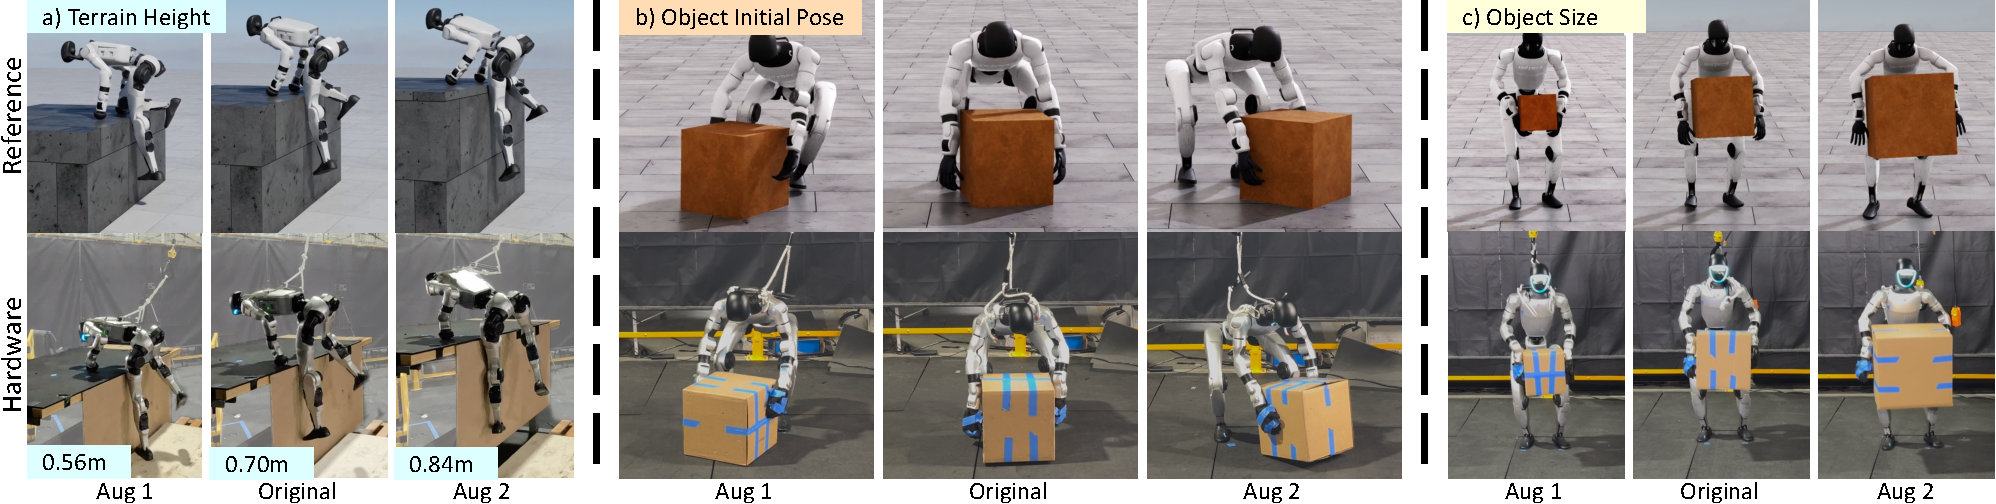
\includegraphics[width=\textwidth]{figures/aug-all-crop.pdf}
	\caption{\label{fig:aug} \OmniRetarget generates systematic variations of (a) terrain height, (b) object initial pose, and (c) object shape from a single human demonstration, with optimized motions in simulation (top) transferring consistently to hardware (bottom). }
	\label{fig:all_aug}
    % \vspace*{-0.4cm}
\end{figure*}

\subsection{Terrain, Object Shape and Spatial Augmentation}
\label{sec:aug}
A key advantage of our framework is its capability for systematic data augmentation, which eliminates the need for collecting numerous, repetitive demonstrations with minor spatial variations. Our method can transform a single human demonstration into a rich and diverse dataset by parametrically altering object configurations, shapes, or terrain features. For each new scenario, we re-solve the optimization problem with fixed $\mathcal{P}_t^{\text{source}}$ and augmented $\mathcal{P}_t$: minimizing the interaction mesh deformation finds a new, kinematically valid robot motion $\{q_t\}$ that preserves the essential spatial and contact relationships of the original interaction.

\textbf{Robot-Object.}
We generate diverse interactions by augmenting both the object's spatial configuration and its shape. 
% We apply rotations and translations to the object's initial pose (Fig. \ref{fig:spatial_aug}), which is then smoothly annealed into the nominal trajectory via an exponential schedule detailed in \eqref{eq:aug_obj_traj}, and scale its dimensions (Fig. \ref{fig:obj_shape_aug}) 
We apply translations and rotations to modify the object's initial pose (Fig. \ref{fig:all_aug}b) and blend the new initial pose with the original object motion via interpolation with an exponential schedule detailed in \eqref{eq:aug_obj_traj}. 
In addition, we scale the three dimensions of the object (Fig. \ref{fig:all_aug}c). A critical component of this process is constructing the interaction mesh in the object's local frame, which ensures that the robot's interacting body parts naturally follow the object's transformation (Sec. \ref{sec:im_in_obj_frame}). 

However, this alone can lead to trivial augmentations where the entire robot undergoes a rigid transformation along with the object. To generate more meaningful data diversity, we introduce cost terms and constraints that anchor parts of the robot's body to the nominal trajectory $\{\bar q_t^\star\}$. For instance, in a pick-up task, we encourage the robot to discover new upper-body coordination by penalizing lower-body deviations from the original motion:
\begin{equation}
    \|q_t - \bar q_{t}^\star\|_W,
\end{equation}
where $W$ heavily penalizes the lower-body entries, constraining the initial foot poses to match the nominal trajectory
\begin{equation}
    p_0^{F} = \bar p_{0}^{F \star} \quad \text{ for left and right feet}.
\end{equation}
These added objectives prevent the optimization from collapsing to a simple rigid transform of the nominal trajectory and instead produce genuinely new and diverse interactions.

\textbf{Robot-Terrain.}
We generate diverse terrain scenarios by scaling environmental features, such as varying the platform height and depth (Fig. \ref{fig:all_aug}a), and introducing additional constraints. For instance, to encourage stable ground contact when the terrain is elevated, we uniformly sample a grid of points on the ground surface into the interaction mesh.


\section{RL Training with Minimal Formulation}
% Having established our method for generating high-quality kinematic reference motions, we now use RL to bridge the gap between kinematics and dynamics. We train a low-level policy to translate these reference trajectories into dynamic, physically-realizable actions, enabling zero-shot deployment from simulation to real-world hardware.

% Reward engineering is a central challenge in RL for humanoid robots. To mitigate artifacts like foot sliding and penetration present in flawed reference motions, prior works~\cite{ze2025twist, he2025asap, li2025reinforcement} often introduce a suite of ad-hoc regularizers (e.g., foot flight and contact time) to mitigate artifacts in retargeted references such as foot sliding and penetration. Tuning these complex reward terms is notoriously tedious and time-consuming.

% In contrast, OmniRetarget yields artifact-free references, allowing us to adopt the minimal RL formulation from BeyondMimic~\cite{liao2025beyondmimic} for motion tracking. This enables us to achieve faithful tracking of dynamic scene interactions and zero-shot sim-to-real transfer without hyperparameter tuning. For brevity, we describe only our modifications to BeyondMimic and refer to the original work for details.
Having established our method for generating high-quality kinematic references, we use RL to bridge the gap to dynamics by training a low-level policy that converts these trajectories into physically realizable actions, enabling zero-shot transfer from simulation to hardware.

Reward engineering is often the main difficulty in humanoid RL: prior works~\cite{ze2025twist, he2025asap, li2025reinforcement} rely on many ad-hoc regularizers (e.g., foot flight and contact time) to compensate for artifacts in noisy references, but tuning these terms is tedious and fragile. In contrast, BeyondMimic~\cite{liao2025beyondmimic} shows that when references are clean~\cite{unitree_lafan1_retargeting_dataset}, a minimal reward is already sufficient for high-quality tracking.
Since OmniRetarget produces such artifact-free, interaction-preserving references, we can follow this minimal formulation directly, achieving faithful tracking of dynamic interactions and zero-shot sim-to-real transfer \emph{without any hyperparameter tuning}. 

% For brevity, we refer to BeyondMimic for details.
\textbf{Observations.} 
% \guanya{bullet points}
% \guanya{can we define policy input more rigorously? $\pi(\cdots)$}
% To test the hypothesis that our high-quality reference motions can serve as a sufficient prior for complex tasks, we intentionally design a minimal, proprioceptive observation space for our RL policy. We exclude all explicit scene and object information, forcing the agent to be blind rely on the learned motor patterns from the reference trajectory. Moreover, for highly agile sequences involving flight phases or significant terrain changes—where global state estimation is often unreliable—we also omit the robot's root linear position and velocity. 
To show that high-quality reference motions provide a sufficient prior for complex tasks, we design a \emph{minimal proprioceptive} observation space, as listed below, where the agent is blind to explicit scene and object information and must follow the reference trajectory precisely. 

\begin{itemize}
    \item \emph{Reference Motion: } Reference Joint Position/Velocity, Reference Pelvis Position/Orientation Error;
    \item \emph{Proprioception: } Pelvis Linear/Angular Velocity, Joint Position/Velocity;
    \item \emph{Previous Action: } Policy action from last timestep. 
\end{itemize}

For agile motions where state estimation is unreliable, we mask out the pelvis linear position error and velocity.

\textbf{Rewards.} 
% \guanya{bullet point} 
To show the benefits of high-quality reference and avoid reward tuning, we use only five reward terms: 
\begin{itemize}
    \item \emph{Body Tracking: } DeepMimic-style tracking term for body position, orientation, linear and angular velocity;
    \item \emph{Object Tracking (where applicable): } DeepMimic-style tracking term for object position and orientation;
    \item \emph{Action Rate: } Penalize rapid changes in action;
    \item \emph{Soft Joint Limit: } Penalize robot joint limit violation;
    \item \emph{Self-Collision: } Binary penalty on each body if its self-collision force exceeds $1$ N.
\end{itemize}
We use the same weights and hyperparameters from~\cite{liao2025beyondmimic} out of the box without tuning. For object tracking, we use the same hyperparameters as body tracking terms. 
% Following ~\cite{liao2025beyondmimic}, we use four terms: whole-body DeepMimic-style tracking, action smoothing, self-collision, and soft joint limits. Using the default hyperparameters without tuning, these suffice for high-quality tracking of scene interactions. For object loco-manipulation, we add object-pose tracking, $r_\text{obj} = e^{- \|q_\text{obj} - q_\text{obj}^*\| / \omega}$, where $q_\text{obj}^*$ is the desired object pose from the reference motion, and $\omega$ is the same standard deviation as in ~\cite{liao2025beyondmimic}. The weight for object-pose tracking is the same as other tracking terms. \guanya{previous work will add extra XXX}


\textbf{Termination.} 
We terminate training episodes with large body tracking deviations~\cite{liao2025beyondmimic}. For object loco-manipulation, episodes terminate when the object deviates more than $1.0\text{m}$ and $45$° from the reference trajectory. We only apply this criterion after the policy achieves reasonable body tracking.

\begin{figure*}
\centering
\includegraphics[width=\textwidth]{figures/results_all_v2_compressed.pdf}
	\caption{Additional hardware results showing diverse, agile and human-like behaviors. }
	\label{fig:results_capacity}
    % \vspace*{-0.3cm}
\end{figure*}


\textbf{Domain Randomization.}
To improve generalization across object properties for a single reference motion, we randomize the object's physical parameters: mass (0.1–2 kg), center of mass (±0.08 m), inertia (50–150\%), and shape (±10\%). 
For the robot specifically, in contrast to the many terms in prior works (e.g., random force injection (RFI), motor PD, action delay), we only apply four terms: 
\begin{itemize}
    \item \emph{Torso COM Position}: $\pm 0.025$ m in $x$, $\pm 0.05$ m in $y$, $\pm 0.075$ m in $z$;
    \item \emph{Joint default position}: $\pm 0.01$ rad;
    \item \emph{Random push}: $0.3$ m/s, $0.78$ rad/s for $(1\text{--}3)$ s;
    \item \emph{Observation noise}: $\pm 0.05$ for orientation in Rot6D, $\pm 0.5$ m/s and $\pm 0.2$ rad/s for linear and angular velocity, $\pm 0.01$ rad and $\pm 0.5$ rad/s for joint position and velocity. 
\end{itemize}
%We randomize ground friction for both robot and object in $[0.1, 0.6]$.
% Combined with the spatial and shape augmentations in Sec.~\ref{sec:aug}, this covers a broad range of object geometries and initial conditions.

\textbf{Policy Training.}
We group similar motions for faster training. All box-moving motions share a single multi-task policy, while platform climbing uses one policy per reference.




\section{Experimental Results}
In this section, we present a comprehensive experimental validation of \OmniRetarget. We first demonstrate the breadth of complex behaviors enabled by our approach, including natural object manipulation and terrain interaction. We then provide a quantitative benchmark against state-of-the-art baselines, evaluating performance across kinematic quality metrics and downstream policy performance.
\subsection{Whole-Body Scene-Object-Interaction} 
\paragraph{Agile Loco-Manipulation}
\OmniRetarget enables RL policies to learn agile, whole-body motions for complex scene interactions and loco-manipulation in simulation, culminating in successful zero-shot sim-to-real transfer to hardware. Shown in Fig.~\ref{fig:results_capacity}, policies trained on our data reproduce a diverse range of expressive behaviors on a Unitree G1 humanoid, including natural box-carrying motions retargeted from the OMOMO dataset, dynamically climbing a $0.9$m-high platform ($70$\% of the robot's height), and crawling over slopes, showing clean and accurate contact sequences. 

To showcase the full capabilities of our framework, we present a long-horizon, dynamic sequence inspired by the Boston Dynamics Atlas tool-use demo \cite{BostonDynamics2023Atlas}. Visualized in Fig.~\ref{fig:flagship_demo}, our retargeted data enables the robot to carry a $4.6$ kg chair to a platform, use it as a stepstone to climb up, and then leap off, performing a parkour-style roll to absorb the landing impact. This 30-second, complex, multi-stage task highlights \OmniRetarget's ability to produce precise and versatile reference motions, pushing the boundaries of what is possible for humanoids learning agile, human-like behaviors.


We additionally showcase a high-dynamic wall-flip motion\footnote{The motion is acquired from \url{https://actorcore.reallusion.com/3d-motion?asset=parkour-tic-tac-backflip}
. An IMU capable of measuring angular rates above $15$ rad/s is required for this motion.} in Fig.~\ref{fig:wallflip}. The robot completes the full flip in approximately $0.5$ second, reaching a peak angular velocity of $15$ rad/s.
Unlike the human foot, which can flex at the arch to maintain contact and generate friction, the robot foot is rigid. As a result, it must align more closely to the wall to achieve sufficient contact area and friction.
To account for this physical difference and give RL more freedom to learn this skill, we relaxed the termination condition during RL training by increasing the end-effector position error threshold to $0.5$ meter (compared to $0.25$ meter used in other motions) and removed the foot joint orientation tracking term from the reward function. All other components of the tracking objective remain consistent with other motions.
The trained policy is robust and achieves a $5/5$ success rate in our real-world experiments.

\begin{figure*}
\centering
\includegraphics[width=\textwidth]{figures/wallflip_v32_compressed.pdf}
	\caption{Hardware results showing a high-dynamic wall-flip motion. The robot reaches a maximum linear velocity of $3.5$ m/s and a peak angular velocity of $15$ rad/s. }
	\label{fig:wallflip}
    % \vspace*{-0.3cm}
\end{figure*}
% \paragraph{Cross-Embodiment Data Generation}

\paragraph{Sim-to-real with Augmented Data} 
We show that the augmented motions from our pipeline can be used for training and deployment effectively. As shown in Fig.~\ref{fig:aug}, the interaction mesh formulation allows \OmniRetarget to generalize a single nominal motion into box-picking across shapes and positions, as well as platform climbing at different heights. Notably, these augmented motions transfer to hardware without reward tuning, effectively expanding the repertoire of scenes and behaviors we can achieve in real.

In comparison, relying solely on domain randomization--which perturbs object shapes and poses only during training--performs poorly under our RL formulation, as the policies struggle to explore far beyond the nominal reference. Policies trained on our augmented data instead yield reliable success (see video for comparison). Admittedly, additional reward engineering could help, but it contradicts our minimal design goal. Quantitatively, training and evaluating on the full augmented dataset achieves a $79.1\%$ success rate, comparable to $82.2\%$ when evaluating on nominal motions only, showing that kinematics augmentation substantially enlarges coverage without significant performance degradation.

% We will open-source this data to support the community in developing natural, diverse interaction skills for humanoid robots.

\begin{table*}[tb]
\centering 
\begin{tabular}{lcccccc} 
\toprule 
& \multicolumn{2}{c}{\textbf{Penetration}} & \multicolumn{2}{c}{\textbf{Foot Skating}} & \textbf{Contact Preservation} &
\textbf{Downstream RL Policy}\\ 
\cmidrule(lr){2-3} \cmidrule(lr){4-5} \cmidrule(lr){6-6} \cmidrule(lr){7-7} 
\textbf{Method} & Duration $\downarrow$ & Max Depth (cm) $\downarrow$ & Duration $\downarrow$ & Max Vel. (cm/s) $\downarrow$ & Duration $\uparrow$ & Success Rate $\uparrow$\\ 
\midrule
\multicolumn{6}{l}{\textit{Robot-Object Interaction (Retargeting from the OMOMO Dataset)}} \\
\midrule 
PHC~\cite{Luo2023PerpetualHC} & 0.68 $\pm$ 0.21 & 5.11 $\pm$ 3.09 & 0.05 $\pm$ 0.05 & 1.40 $\pm$ 0.80 & 0.96 $\pm$ 0.09 & 71.28\% $\pm$ 22.55\%\\ 
GMR~\cite{ze2025twist} & 0.83 $\pm$ 0.14 & 8.50 $\pm$ 3.94 & 0.02 $\pm$ 0.01 & 1.46 $\pm$ 0.45 & \textbf{0.99 $\pm$ 0.04} & 50.83 \% $\pm$ 23.89\% \\  
VideoMimic~\cite{videomimic} & 0.60 $\pm$ 0.27 & 7.48 $\pm$ 4.95 & 0.12 $\pm$ 0.07 & 1.50 $\pm$ 0.70 & 0.77 $\pm$ 0.25 & 3.85\% $\pm$ 8.41\%\\ 
\OmniRetarget & \textbf{0.00 $\pm$ 0.01} & \textbf{1.34 $\pm$ 0.34} & \textbf{0} & \textbf{0} & 0.96 $\pm$ 0.09 & \textbf{82.20\% $\pm$ 9.74\%}\\
\midrule
\multicolumn{6}{l}{\textit{Robot-Terrain Interaction (Retargeting from the In-House MoCap Dataset)}} \\
\midrule
PHC & 0.66 $\pm$ 0.36 & 7.74 $\pm$ 4.53 & 0.15 $\pm$ 0.04 & 2.03 $\pm$ 1.83 & 0.45 $\pm$ 0.28 & 52.63\% $\pm$ 49.93\% \\ 
GMR & 0.91 $\pm$ 0.16 & 5.72 $\pm$ 3.84 & 0.04 $\pm$ 0.05 & 1.75 $\pm$ 3.01 & 0.67 $\pm$ 0.26 & 78.94\% $\pm$ 40.77\% \\ 
VideoMimic & 0.83 $\pm$ 0.11 & 5.97 $\pm$ 3.58 & 0.14 $\pm$ 0.05 & 1.85 $\pm$ 1.38  & 0.47 $\pm$ 0.25 & 51.75\% $\pm$ 49.23\% \\ 
\OmniRetarget & \textbf{0.01 $\pm$ 0.02} & \textbf{1.37 $\pm$ 0.18} & \textbf{0} & \textbf{0} & \textbf{0.72 $\pm$ 0.19} & \textbf{94.73\% $\pm$ 22.33\%}\\ 
\midrule
\multicolumn{6}{l}{\textit{Robot-Only (Retargeting from the LAFAN1 Dataset)}} \\
\midrule
Unitree~\cite{unitree_lafan1_retargeting_dataset} & 0.09 $\pm$ 0.13 & 3.22 $\pm$ 2.64 & 0.06 $\pm$ 0.03 & 1.46 $\pm$ 0.01 & N/A & \textbf{100\%} \\
\OmniRetarget & \textbf{0.00 $\pm$ 0.00} & \textbf{1.07 $\pm$ 0.00} & \textbf{0} & \textbf{0} & N/A & \textbf{100\%} \\
\bottomrule 
\end{tabular}
\caption{\label{tab:kinematic_quality} Quantitative comparison of kinematic retargeting quality and downstream RL performances.}
\vspace{-0.4cm}
\end{table*}


\subsection{Benchmark Against Prior Retargeting Pipelines}
\begin{figure}
\centering
\includegraphics[width=0.48\textwidth]{figures/baseline-comparison-crop.pdf}
	\caption{\label{fig:artifact}Artifacts resulting from the retargeting baselines. 
    % \lujie{Highlight penetration with red circles. Make box transparent to show depth of penetration and robot configuration behind the box.}
    }
	\label{fig:baseline_artifacts}
    \vspace*{-0.4cm}
\end{figure}

We compare \OmniRetarget against several widely-used open-source retargeting baselines\footnote{Baseline performance may depend on their hyperparameters. We initialized from the default settings in their public codes, and further improved to ensure consistent performance across different tasks.}: PHC~\cite{Luo2023PerpetualHC}, GMR~\cite{ze2025twist} and VideoMimic~\cite{videomimic}. The generated dataset including 2.78 hours of box carrying in OMOMO, 1 hour of in-house MoCap and 4.6 hours of LAFAN1 will be open-sourced. 
%, which uses the PyRoki~\cite{kim2025pyroki} library. 
\paragraph{Kinematics Quality} We evaluate the kinematic quality of retargeted motions on a Unitree G1 with three criteria:
\begin{enumerate}
    \item \textbf{Penetration}: Measured by the time duration (normalized by the trajectory length) and maximum depth of intersections between the robot, objects, and terrain.
    \item \textbf{Foot Skating}: Quantified by the time duration (normalized by the total desired foot sticking length) and maximum skating velocity of a stance foot.
    \item \textbf{Contact Preservation}: Quantified by the time duration (normalized by the desired contact length). For \textit{robot-object} tasks, we measure hand-object contact. For \textit{robot-terrain} tasks, we measure contact between the robot's hands, toes, and heels with the terrain surface.
\end{enumerate}
As illustrated in Tab.~\ref{tab:kinematic_quality}, \OmniRetarget significantly outperforms all baselines across most kinematic metrics. While \OmniRetarget occasionally incurs minor penetration due to the linearization of constraints \eqref{eq:non-penetration_cstr} in the sequential SOCP solver, the violations are minimal and can be efficiently fixed by RL. 
% and do not significantly affect the RL training. 
GMR achieves the highest contact preservation score for robot-object interaction tasks; however, this outcome largely reflects its keypoint-matching objective. In practice, scaling human hand keypoints to the robot’s size often drives the robot’s hands inside the object, leading to substantial penetration errors (Fig. \ref{fig:baseline_artifacts}b). Overall, all baselines exhibit significant penetration and foot skating (Fig. \ref{fig:baseline_artifacts}), degrading the downstream RL performance, as discussed next.

For a direct comparison on pure locomotion, we retarget motions from the LAFAN1 MoCap dataset \cite{harvey2020robust} and benchmark them against the publicly available Unitree LAFAN1 retargeted dataset \cite{unitree_lafan1_retargeting_dataset}. This serves as a strong baseline, as it is widely considered a high-quality data source for RL-based locomotion training~\cite{liao2025beyondmimic}. Table~\ref{tab:kinematic_quality} shows that \OmniRetarget's motions exhibit fewer physical artifacts, achieving better satisfaction of hard constraints.
% PHC exhibits the most violations foot skating and a lot of penetration. GMR improves by using a better optimizer (Mink) but still suffers from penetration issues. VideoMimic reduces penetration by including it in constraints but has large contact preservation errors due to treating penetration separately from interaction dynamics. In contrast, \OmniRetarget achieves minimal constraint violations and the highest contact preservation, demonstrating the advantage of the interaction mesh formulation that preserves interaction dynamics rather than merely matching keypoints.



\paragraph{Downstream RL Performance}
\label{sec:downstream-rl}
A central observation from prior works~\cite{liao2025beyondmimic, zhang2025hub} is that the quality of retargeted motions strongly influences the performance of downstream RL. To verify this, we select 39 challenging motions for \OmniRetarget and baselines, and train RL policies using identical hyperparameters from~\cite{liao2025beyondmimic} without manual tuning. We evaluate the policies in simulation, and success is measured by training termination criteria.

Shown in Tab.~\ref{tab:kinematic_quality}, retargeting quality directly impacts RL success rates. \OmniRetarget consistently achieves the highest performance across tasks, exceeding baselines by over 10\% with lower variance, which indicates more stable learning across different motions. PHC performs better than GMR in object manipulation, likely due to lower penetration with sufficient contact preservation, but worse in terrain interaction, where its contact preservation drops by nearly 50\%. Specifically for terrain interaction, we see that contact preservation is directly proportional to the success rate. These results suggest that both contact preservation and penetration reduction are critical for generalizing RL policies across diverse tasks, and \OmniRetarget shows strength in both.

VideoMimic shows the weakest interaction preservation among all baselines (Fig.~\ref{fig:artifact}c), likely due to its collision avoidance soft cost conflicting with the keypoint matching cost. 
% For example, a hand can satisfy a proximity target to a keypoint while being on the wrong side of an object. 
This is compounded by its coarse collision model originally designed for heightmaps, which is ill-suited for precise loco-manipulation. Consequently, while its terrain-interaction results are comparable to PHC, its performance on object manipulation is poor. Although this could be partially attributed to the tuning of its soft penalties, \OmniRetarget demonstrates that a hard-constraint formulation avoids such sensitivities altogether. 
% In contrast, VideoMimic shows the weakest interaction preservation among the methods (Fig.~\ref{fig:artifact}c). This underscores the need to preserve interactions explicitly: while other baselines maintain a coarse structure, VideoMimic often pushes the motion too far from the object, especially since keypoint matching (proximity to a keypoint) does not ensure the correct spatial relationship (e.g., a hand meant for the side of a box may end up behind it). In addition, it only adopts a coarse collision model originally designed for heightmaps. These factors result in poor performance for object manipulation, though its terrain-interaction results are comparable to PHC. To be fair, some of this may be due to limited tuning of its soft penalties. Nonetheless, \OmniRetarget avoids such sensitivity by not relying on soft constraints.

% \paragraph{Kinematics Augmentation v.s. Domain Randomization}

% \begin{figure}
% \centering
% \includegraphics[width=0.48\textwidth]{figures/aug-dr-crop.pdf}
% 	\caption{\label{fig:augdr} Comparison of object shape and initial pose augmentation in kinematics stage vs. training-only randomization.
%     }
% 	\label{fig:terrain_aug}
%     \vspace*{-0.6cm}
% \end{figure}
% \begin{table}
% \centering 
% \begin{tabular}{lccc} 
% \toprule 
% & \multicolumn{3}{c}{\textbf{Success Rate}} \\ 
% \cmidrule(lr){2-4}
% \textbf{Method} & Object Picking & Terrain Climbing & Crawling \\ 
% \midrule 
% PHC &   &    &    \\ 
% GMR &    &    &  \\ 
% VideoMimic &    &    &    \\ 
% \OmniRetarget & \textbf{  } & \textbf{  } & \textbf{} \\
% \bottomrule 
% \end{tabular}
% \caption{\label{tab:rl_success_rate} Success rate of downstream RL policies for robot-object and robot-terrain interactions.}
% \end{table}

% \paragraph{Sim-to-real Evaluation}
% To avoid damaging the hardware, we select the best baseline, GMR, to retarget a challenging wall-climbing motion for comparison with \OmniRetarget. Shown in Fig.~\ref{}, although GMR’s policy learns successfully in simulation, it exhibits unnatural knee shaking to compensate for inaccurate retargeting, resulting in less robust behavior that fails on real hardware.



\section{Conclusion}
% \guanya{future work: jointly optimize the whole trajectory, handle noisy motions, learning autonomous policies, etc}

In this work, we tackled a key data bottleneck caused by a lack of high-quality, interaction-aware retargeting pipeline in humanoid whole-body loco-manipulation. 
We introduced \OmniRetarget, a unified, interaction-preserving data generation engine that leverages an interaction mesh within a single constrained optimization. Our experiments showed that \OmniRetarget significantly outperforms prior methods in kinematic quality, producing a diverse set of artifact-free trajectories from single demonstrations. 
This high-quality data enabled a proprioceptive RL policy, trained with minimal formulation, to achieve long-horizon dynamic skills on a physical humanoid via zero-shot sim-to-real transfer.

Ultimately, \OmniRetarget demonstrates a paradigm shift from patching lower-quality reference motions with complex reward engineering to solving the problem at its source with principled data generation. While our current frame-by-frame optimization is mostly effective, future work could explore jointly optimizing the entire trajectory to enhance the framework's robustness to noisier motion sources, such as video data, or learning autonomous visuomotor policies. By open-sourcing our complete framework and the large-scale dataset of retargeted trajectories, we hope to accelerate progress towards more agile, capable, and versatile humanoid robots. \looseness=-1

\begin{small}
\bibliography{IEEEabrv, root}
\bibliographystyle{IEEEtran}
\end{small}

% \clearpage
\section*{APPENDIX}
\subsection{Different Sources of Human Motion Data}
% Human motion datasets contain rich pose and shape information but come in various formats that require standardization before use in a retargeting pipeline. 
% The primary goal of preprocessing is to convert these diverse formats into a consistent representation—typically a time series of global 3D keypoint positions $\{p^\text{source}_{0:T, i}\}$. This process must also account for morphological differences between the human demonstrator and the target robot. 
Human motion datasets contain rich pose and shape information, but they differ both in data format and in the physical attributes (e.g., height, body proportions) of the demonstrators. To make them compatible across different sources and suitable for retargeting, we need to convert these inputs into a consistent representation, typically a time series of global 3D keypoint positions $\{p^\text{source}_{0:T, i}\}$. This process must account for differences between human demonstrators and the target robot.

The datasets used in this work represent two common formats:
\begin{itemize}
    \item \textbf{Parametric Human Models}: The OMOMO dataset uses the SMPL format \cite{SMPL:2015}, a parametric model representing human body shape and pose-dependent variations using shape ($\beta$) and pose ($q$) parameters.
    \item \textbf{Skeleton Hierarchy}: Both our in-house MoCap data and the LAFAN1 dataset utilize the skeleton hierarchy defined in the BVH format.
\end{itemize}
Different retargeting pipelines use different strategies to handle these formats. We detail these preprocessing steps below, denoting the human demonstrator's pose as $q^\text{demo}_{t}$, the SMPL forward model for the $i$-th keypoint as $M_i$, the original demonstrator shape as $\beta^{\text{demo}}$, and the demonstrator's $i$-th keypoint position as $p^\text{demo}_{t,i}$.


\subsubsection{SMPL Data}
To handle data from parametric models like SMPL, methods typically follow one of two strategies: fitting the model to the robot's morphology or directly scaling the human's keypoints.
\begin{algorithm}
\caption{Fit SMPL Shape (PHC)}
\begin{algorithmic}[1]\label{alg:phc_fit_smpl_shape}
\REQUIRE SMPL model $M$, robot urdf with forward kinematics $f$, $\bar q^\text{smpl} = 0_{n_s}, \bar q^\text{robot} = 0_{n_x}$
\ENSURE scaling factors $\alpha, \beta$
\STATE $\alpha, \beta \leftarrow 1, 0_{10}$
\FOR{$\text{iter} = 1, \ldots, \text{max\_iter}$}
    \STATE $L(\alpha, \beta) = \sum_i \left\|(f_i(\bar q^\text{robot}) - \alpha \cdot M_i(\bar q^\text{smpl}; \beta)\right\|^2$
    \STATE $\alpha \leftarrow \alpha - \eta_{\alpha} \cdot \nabla_{\alpha} L$
    \STATE $\beta \leftarrow \beta - \eta_{\beta} \cdot \nabla_{\beta} L$
\ENDFOR
\end{algorithmic}
\end{algorithm}
\paragraph{Model Fitting (PHC, VideoMimic)} This strategy fits a scaled SMPL model to the robot's morphology. PHC first optimizes for an overall scaling factor $\alpha$, and a set of SMPL shape parameters $\beta$ that best match the robot's link length in a canonical T-pose, as detailed in Alg. \ref{alg:phc_fit_smpl_shape}. The final source keypoint positions are then generated from this fitted model:\looseness=-1
\begin{equation}
p^\text{source}_{t,i} = \alpha \cdot M_i(q^\text{demo}_t; \beta).
\end{equation}
VideoMimic adopts a similar philosophy but integrates the scaling directly into its main retargeting optimization, solving for per-link scale factors jointly with the robot's motion.
% \begin{itemize}
%     \item \textbf{Model Fitting:} PHC and VideoMimic fit a scaled SMPL model to the robot's morphology by optimizing shape parameters $\beta$ and a scaling factor $\alpha$.
%     \item \textbf{Direct Scaling:} GMR and OmniRetarget directly extract keypoint positions from the human's SMPL parameters and scale them to the robot's size, often using a height ratio.
% \end{itemize}


\paragraph{Direct Scaling (GMR \& \OmniRetarget)}
In contrast, GMR and \OmniRetarget use a more direct approach. They generate keypoints from the human's \emph{original} SMPL parameters $\beta^{\text{demo}}$ and then scale them to the robot's proportions. 
Both methods support detailed morphological adaptation via per-bone scaling factors based on corresponding human-robot link lengths. For simplicity in this work, however, we adopt a single global scaling factor $\alpha$, set to the robot-to-human height ratio:
% To scale each link correctly for inverse kinematics, GMR requires manual tuning of per-bone scaling factors based on the corresponding human–robot link length ratios. In essence, GMR fits a human model onto the robot's shape manually. 

% In contrast, OmniRetarget does not require using an exact human model to begin with, thus avoiding this tedious process and only needs a single global scaling factor, $\alpha$, defined as the robot-to-human height ratio:
\begin{equation}\label{eq:gmr_scaling}
    p^\text{source}_{t,i} = \alpha \cdot M_i(q^\text{demo}_t; \beta^{\text{demo}}), \alpha=\frac{h_{\text{robot}}}{h_{\text{demo}}}.
\end{equation}

\begin{table*}[tb]
\centering
\begin{tabular}{@{}lllll@{}}
\toprule
\textbf{Method} & \textbf{Optimization Type} & \textbf{Primary Objective} & \textbf{Preprocessing} & \textbf{Data Formats} \\ \midrule
PHC & Trajectory-wise Optimization & Keypoint Position Matching & Model Fitting & SMPL \\
GMR & Per-Frame Optimization & Keypoint Position \& Orientation Matching  & Direct Scaling & SMPL, BVH  \\
VideoMimic & Trajectory-wise Optimization & Pairwise Distance \& Orientation Preservation & Model Fitting & SMPL \\
IMMA & Multi-Stage Trajectory-wise Optimization & Interaction Mesh Deformation + IK & Unknown & Unknown \\ \midrule
\textbf{\OmniRetarget} & Per-Frame Optimization & Interaction Mesh Deformation & Direct Scaling & SMPL, BVH   \\ \bottomrule
\end{tabular} 
\caption{\label{tab:method_comparison}Comparison of different retargeting methodologies}
\end{table*}

\subsubsection{Skeleton Hierarchy Data}
For formats like BVH, keypoint positions are derived from the skeleton's forward kinematics $f^\text{skeleton}$. This data is then typically scaled to the robot's size using the height ratio:
\begin{equation}
    p^\text{source}_{t, i} = \frac{h_{\text{robot}}}{h_{\text{demo}}} \cdot f_i^\text{skeleton}(q^\text{demo}_t).
\end{equation}

A key distinction among methods is their data compatibility. While GMR and \OmniRetarget are designed to process both parametric model data and raw skeleton hierarchies, frameworks like PHC and VideoMimic are primarily designed for SMPL data. Fitting other data formats to the SMPL format is yet another tedious process. 

\subsection{Different Kinematic Retargeting Formulations}
Once human motion is preprocessed into a series of source keypoint positions $\{p^\text{source}_{0:T, i}\}$, different methods formulate the retargeting problem in distinct ways. As summarized in Tab.~\ref{tab:method_comparison}, these approaches vary in their optimization strategy and objectives. The following sections detail the mathematical formulation of each baseline method and our proposed approach, \OmniRetarget.
% As mentioned in Sec. \ref{sec:motion_retargeting}, researchers have adopted various formulations to retarget human motions to robot trajectories. PHC uses keypoint matching, while GMR extends this approach to match both keypoint positions and orientations. VideoMimic preserves the pariwise distance and orientation between keypoint pairs.
\begin{algorithm}
\caption{Retarget Robot Motion (PHC)}
\begin{algorithmic}[1]\label{alg:phc_fit_robot_motion}
\REQUIRE Robot urdf, source keypoint positions $\{p^\text{source}_{0:T, i}\}$
\ENSURE $q_{0:T}$
\STATE $q_{0:T} \leftarrow [0_{n_x}]_T$
\FOR{$\text{iter} = 1, \ldots, \text{max\_iter}$}
    \STATE $\mathcal{L}(q_{0:T}) = \sum_{t=0}^T  \sum_i \left\|f_i(q_t) - p^\text{source}_{t, i}\right\|^2$
    \STATE $q_{0:T} \leftarrow \text{clamp}(q_{0:T} - \nabla_{q_{0:T}} \mathcal{L}(q_{0:T}), q_{\min}, q_{\max})$
\ENDFOR
\end{algorithmic}
\end{algorithm}

\subsubsection{PHC}
PHC formulates retargeting as a large-scale trajectory-wise optimization problem. It applies gradient descent to minimize the error between the source keypoint positions and the robot's keypoint positions over the entire trajectory, as shown in Alg.~\ref{alg:phc_fit_robot_motion}. \looseness=-1



\subsubsection{GMR}
GMR performs retargeting by solving an inverse kinematics (IK) problem at each frame (\ref{alg:gmr_retarget_robot_motion}).
At each timestep, GMR finds the robot configuration $q_t$ that matches the source keypoint positions and orientations via the following optimization program:
\begin{equation} \label{eq:gmr_qp}
    \begin{aligned}
        q_t^\star = \argmin_{q_t} & \sum_i \left\|f_i^p(q_t) - p^\text{source}_{t, i}\right\|^2 + \left\|f_i^\theta(q_t) - \theta^\text{source}_{t, i}\right\|^2 \\
      \text{s.t. } & q_{\min} \leq q_t \leq q_{\max},
    \end{aligned}
\end{equation}
where $f_i^p$ and $f_i^\theta$ are the robot forward kinematics for the $i$-th keypoint's position and orientation, respectively. Leveraging the mink \cite{Zakka_Mink_Python_inverse_2025} library, GMR solves this program in a Sequential Quadratic Programming fashion.
\begin{algorithm}
\caption{Retarget Robot Motion (GMR)}
\begin{algorithmic}[1]\label{alg:gmr_retarget_robot_motion}
\REQUIRE Robot urdf, source keypoint positions $\{p^\text{source}_{0:T, i}\}$ and orientations $\{\theta^\text{source}_{0:T, i}\}$
\ENSURE $q_{0:T}$
\FOR{$t = 0, \ldots, T$}
    \STATE $q_{t} \leftarrow$ Solve IK \eqref{eq:gmr_qp}
\ENDFOR
\end{algorithmic}
\end{algorithm}

\subsubsection{VideoMimic}
% VideoMimic performs a joint optimization over the robot's trajectory $q_{0:T}$ and per-link scaling factors $\beta_{ij}$. Its primary objective is to preserve the scaled pairwise distances and orientations between keypoints. The full objective includes multiple penalty terms for physical constraints:

VideoMimic jointly optimizes for the robot motion $q_{0:T}$ and SMPL per-link scaling factor $\beta$ over the entire trajectory. The primary objective is to preserve the scaled pairwise distance and orientation between each keypoint pair $(i, j)$:
\begin{equation}
    \mathcal{L}_{\text{pairwise}} = \sum_{t, i \in \mathcal{N}(j)} \|\beta_{ij} \cdot (p^\text{demo}_{t,i} -  p^\text{demo}_{t,j}) - (f_i(q_t) - f_j(q_t))\|_2^2,
\end{equation}
with soft penalties on foot contact matching $\mathcal{L}_{\text{contact}}$, foot skating $\mathcal{L}_{\text{skating}}$, collision $\mathcal{L}_{\text{collision}}$, joint limits $\mathcal{L}_{\text{joint}}$ and temporal smoothness $\mathcal{L}_{\text{smooth}}$:
\begin{equation} \label{eq:videomimic_opt}
    \begin{aligned}
        q_{0:T}^\star, \beta^\star = & \argmin_{q_{0:T}, \beta} \quad  \mathcal{L}_{\text{pairwise}} + \lambda_c \cdot \mathcal{L}_{\text{contact}} + \lambda_s \cdot \mathcal{L}_{\text{skate}} + \\
        & \lambda_{cl} \cdot \mathcal{L}_{\text{collision}} + \lambda_j \cdot \mathcal{L}_{\text{joint}} + \lambda_{sm} \cdot \mathcal{L}_{\text{smooth}} + \ldots
    \end{aligned}
\end{equation}
\begin{algorithm}
\caption{Retarget Robot Motion (VideoMimic)}\label{alg:videomimic_retarget}
\begin{algorithmic}[1]
\REQUIRE Robot urdf, demonstrator's original keypoint positions $\{p^\text{demo}_{0:T, i}\}$
\ENSURE $q_{0:T}, \beta$ $\leftarrow$ Solve \eqref{eq:videomimic_opt} for the entire trajectory
\end{algorithmic}
\end{algorithm}

\subsubsection{IMMA Multi-stage Optimization}
IMMA relies on a complex, multi-stage pipeline: first, it optimizes the intermediate robot keypoint positions to warp the interaction mesh from the human to the robot with minimal deformation by solving the following program
\begin{equation}
    \begin{aligned}
    p_{t,i}^\star = \argmin_{p_{t_i}} \quad & \sum_{i} \|L(p_{t,i} ^{\text{source}})-L(p_{t,i})\|^2 \\
    \text{s.t.} \quad & \phi_j(q_t) \geq 0, \forall j \\
    & \|p_{t,i} - p_{t,j}\|_2 = l_{ij}, \forall \text{bone} \\
    & p_t^{F} = p_{t-1}^{F}, \forall \text{stance foot}, 
\end{aligned}
\end{equation}
where $l_{ij}$ is the bone length between the $i$-th and $j$-th joints. Then, it solves a separate IK problem to recover joint angles that best match the intermediate keypoints: 
\begin{equation}
    \begin{aligned}
        q_t^\star = \argmin_{q_t} \sum_i \|f_i(q_t) - p_{t,i}^\star \|_2^2.
    \end{aligned}
\end{equation}
In later stages, additional hard constraints on the feet and waist are imposed to prevent foot slipping and ensure dynamic balancing. This sequential and fragmented approach produces dynamically consistent motions but fails to consider crucial kinematic constraints like joint and velocity limits.

\begin{algorithm}
\caption{Retarget Robot Motion (\OmniRetarget)}
\begin{algorithmic}[1]\label{alg:omniretarget_retarget_robot_motion}
\REQUIRE Robot urdf, source keypoint positions $\{p^\text{source}_{0:T, i}\}$
\ENSURE $q_{0:T}$
\FOR{$t = 0, \ldots, T$}
    \STATE $q_{t} \leftarrow$ Solve interaction mesh optimization \eqref{eq:interaction_mesh_opt}
\ENDFOR
\end{algorithmic}
\end{algorithm}

\subsubsection{\OmniRetarget}
\OmniRetarget, as outlined in Alg. \ref{alg:omniretarget_retarget_robot_motion}, operates frame-by-frame by minimizing the Laplacian deformation of the interaction meshes. The core objective \eqref{eq:interaction_mesh_cost} is flexible and can be augmented with task-specific costs, such as the orientation matching term from GMR, providing a unified and extensible framework for motion retargeting.


\subsection{Data Augmentation Details}
% We denote the time step where the box starts moving as $t_m$, the time constants for translational and rotational exponential decay as $\tau_p$ and $\tau_\theta$ respectively. The exponential interpolation scheme for the augmented object trajectory is
% \begin{subequations}\label{eq:aug_obj_traj}
% \begin{align}
% \tilde{p}_{obj}[t] &=
% \left\{
% \begin{aligned}
% & \Delta p_{obj} + p_{obj}[0] \\
% & \hfill \text{(before object starts moving)} \\[2pt]
% & \Delta p_{obj}\, e^{-(t-t_m)/\tau_p} + p_{obj}[t] \\
% & \hfill \text{(after object starts moving)}
% \end{aligned}
% \right. \\[0.75em]
% \tilde{\theta}_{obj}[t] &=
% \left\{
% \begin{aligned}
% & \Delta \theta_{obj} + \theta_{obj}[0] \\
% & \hfill \text{(before object starts moving)} \\[2pt]
% & \Delta \theta_{obj}\, e^{-(t-t_m)/\tau_{\theta}} + \theta_{obj}[t] \\
% & \hfill \text{(after object starts moving)}
% \end{aligned}
% \right.
% \end{align}
% \end{subequations}
\subsubsection{Augmented Object Trajectory}\label{sec:aug_obj_traj}
To generate a perturbed object trajectory, we introduce a transient offset that decays exponentially over time. Let the original trajectory be denoted by $(p_{obj}(t), \theta_{obj}(t))$. We define an initial positional offset $\Delta p_{obj}$ and rotational offset $\Delta \theta_{obj}$ that are applied at the onset of object motion, $t_m$. The augmented trajectory, $(\tilde{p}_{obj}(t), \tilde{\theta}_{obj}(t))$, is then formulated as:

\begin{subequations}\label{eq:aug_obj_traj}
\begin{align}
\tilde{p}_{obj}(t) &=
\begin{cases}
\Delta p_{obj} + p_{obj}(0) & \text{if } t < t_m \\
\Delta p_{obj}\, e^{-(t-t_m)/\tau_p} + p_{obj}(t)& \text{if } t \ge t_m
\end{cases}
\\[0.75em]
\tilde{\theta}_{obj}(t) &=
\begin{cases}
\Delta \theta_{obj} \oplus \theta_{obj}(0) & \text{if } t < t_m \\
\Delta \theta_{obj}\, e^{-(t-t_m)/\tau_{\theta}} \oplus \theta_{obj}(t) & \text{if } t \ge t_m
\end{cases}
\end{align}
\end{subequations}
where $\tau_p$ and $\tau_\theta$ are time constants governing the rate of decay for the translational and rotational perturbations, respectively. The $\oplus$ operator denotes composition for orientations (e.g., quaternion multiplication).


\subsubsection{Interaction Mesh Construction in Object Frame} \label{sec:im_in_obj_frame}
For robot-object interactions, it is crucial to construct the interaction mesh in the object's local coordinate frame. This ensures that the Laplacian coordinates, which encode relative spatial relationships, are invariant to the object's global rotation and translation. As illustrated in Fig. \ref{fig:obj_frame_im}, when the object rotates by \ang{180} (indicated by the black arrow), the Laplacian coordinate of the object in the world frame $L_W$ changes from $(0, 1)$ to $(0, -1)$, while the Laplacian coordinate calculated in the object frame $L_O$ remains constant. Using object-frame coordinates is therefore essential for preserving the intended interaction geometry during object spatial transformation.
\begin{figure}
\centering
\includegraphics[width=0.20\textwidth]{figures/obj_frame_im.png}
	\caption{The Laplacian coorinate should stay the same when the object rotates \ang{180}. }
	\label{fig:obj_frame_im}
    \vspace*{-0.4cm}
\end{figure}

\begin{figure}
\centering
\includegraphics[width=0.23\textwidth]{figures/interaction_mesh.png}
	\caption{The actual target (left) and source (right) interaction meshes used for optimization.}
    % \ak{btw, this figure is very similar to the original paper in that it's about a link but since the paper is about human object interaction I think it would be better with two long arms holding a box that has to be regarted to two shorter arms + box }
	\label{fig:interaction_mesh}
    \vspace*{-0.4cm}
\end{figure}
\subsection{Sequential SOCP Details}
At each time step $t$, we iteratively solve a Second-Order Cone Program (SOCP) for the optimal change in the robot's configuration $dq$ util convergence for up to 10 iterations. For conciseness, we omit the time index $t$ for variables within the Sequential SOCP loop. 

The optimization finds the increment $dq_n$ at the $n$-th iteration. The configuration is updated using this increment, starting from the previous time step's solution ($\bar q_0 = q_{t-1}^\star$):
$$\bar q_{n+1} = \bar q_n + dq_n^\star.$$
The optimal increment $dq_n^\star$ is the solution to the following SOCP, which is linearized around the current iterate  
$\bar q_n$:
\begin{subequations}
\begin{align}
    dq_n^\star = \argmin_{dq_n} \quad & \|L^{\text{source}} - (J_L^n\cdot dq_n +\bar L_n^{\text{target}})\|^2 \\
    & + \|\bar{q}_n + dq_n - q_{t-1}\|_{Q}^2 \\
    \text{s.t.} \quad & J_j^n \cdot dq_n + \phi_j(\bar{q}_n) \geq 0, \forall j \\
    & q_{\min} \leq \bar{q}_n + dq_n \leq q_{\max} \\
    & v_{\min} \cdot dt \leq \bar{q}_n + dq_n - q_{t-1} \leq v_{\max} \cdot dt \\
    & p_t^{F}(\bar{q}_n) + J_{F}^n \cdot dq_n = p_{t-1}^{F}, \forall \text{stance foot} \\
    & \|dq_n\|_2 \leq \epsilon, \label{eq:trust_region_cstr}
\end{align}
\end{subequations}
where 
\begin{itemize}
    \item $L^{\text{source}} = vec(\{L(p_{t,i}^{\text{source}})\})$
    \item $L^{\text{target}}(q) = vec(\{L(p_{t,i}^{\text{target}}(q))\})$
    \item $\bar L_n^{\text{target}} = vec(\{L( p_{t,i}^{\text{target}}(\bar q_n))\})$
    \item $J_L^n = \partial L^\text{target}/\partial q|_{q=\bar q_n}$
    \item $J_j^n = \partial \phi_j/\partial q|_{q=\bar q_n}$
    \item $J_F^n = \partial p_t^F /\partial q|_{q=\bar q_n}$.
\end{itemize}
The second-order cone constraint \eqref{eq:trust_region_cstr} is a trust region constraint with radius $\epsilon$ (we use $\epsilon=0.2$) that keeps the step size small, ensuring the linear approximations remain valid.



\subsection{Downstream RL Evaluation Breakdown}
Shown in Fig.~\ref{fig:histogram}, we present histograms from the downstream RL evaluation (Sec.~\ref{sec:downstream-rl}) to illustrate failure patterns and variance across OmniRetarget and baselines. These histograms break down failure rates by each motion for two tasks: robot–object interaction and robot–terrain interaction, highlighting not only overall averages but also how failures distribute across different motions. We do not include augmented motions as baselines do not support augmentation. 

\begin{figure}
\centering
\includegraphics[width=0.49\textwidth]{figures/histo-crop.pdf}
	\caption{Histograms from the downstream RL evaluation showing the failure patterns for the baselines in different tasks. }
    % \ak{btw, this figure is very similar to the original paper in that it's about a link but since the paper is about human object interaction I think it would be better with two long arms holding a box that has to be regarted to two shorter arms + box }
	\label{fig:histogram}
    \vspace*{-0.4cm}
\end{figure}

In robot–object interaction, the motions are modest while object properties are heavily randomized. Since the motions are not aggressive, most policies can adapt even to low-quality references and achieve at least one success, except VideoMimic, which fails systematically due to poor interaction preservation. This task therefore measures robustness rather than accuracy. We see that GMR shows broader failure spread with lower success rates, likely due to penetration issues that reduce robustness under placement changes. PHC shows improved robustness, while OmniRetarget achieves the most robust performance, with results concentrated in the high-success region.

In contrast, climbing terrains requires much more agile and challenging motions and thus, demands precise reference motions: if the quality is low, the agent fails outright with no successes. Here, PHC and VideoMimic perform the worst, with nearly half the motions failing entirely. GMR delivers somewhat better references but still fails on four motions, while OmniRetarget fails on only one. These results show that OmniRetarget not only provides superior robustness under variation but also higher reference accuracy.

For the one remaining failure, we believe that it is limited by the simple RL formulation we use. For future work, an interesting direction could be to extend the current RL formulation with curriculum learning to support these extremely difficult motions. 
\end{document}
